%====================================================
\section{Thiết kế API}
%====================================================

Trong hệ thống SEAL Hackathon Management System, các chức năng của hệ thống được xây dựng theo kiến trúc RESTful API sử dụng framework FastAPI. Việc lựa chọn mô hình RESTful giúp phân tách rõ ràng giữa giao diện người dùng (Frontend) và tầng xử lý nghiệp vụ (Backend), đồng thời tạo điều kiện thuận lợi cho việc phát triển, bảo trì và mở rộng hệ thống trong tương lai. Dữ liệu trao đổi giữa các thành phần được biểu diễn dưới định dạng JSON nhằm đảm bảo tính thống nhất và khả năng tương thích với nhiều nền tảng khác nhau.

FastAPI được lựa chọn làm nền tảng phát triển Backend nhờ khả năng xử lý bất đồng bộ (Asynchronous), tốc độ thực thi cao và tích hợp sẵn cơ chế sinh tài liệu API thông qua Swagger UI. Nhờ đó, các API của hệ thống có thể được kiểm thử trực tiếp trên trình duyệt mà không cần sử dụng các công cụ hỗ trợ khác. Điều này giúp giảm đáng kể thời gian phát triển và kiểm thử trong quá trình xây dựng hệ thống.

Để đảm bảo tính bảo mật, toàn bộ các API yêu cầu người dùng phải xác thực đều sử dụng cơ chế JWT (JSON Web Token). Sau khi người dùng đăng nhập thành công, hệ thống sẽ tạo một Access Token chứa các thông tin định danh của người dùng như mã tài khoản, vai trò và thời gian hết hạn. Token này sẽ được gửi kèm trong Header của các yêu cầu tiếp theo nhằm xác minh danh tính người dùng trước khi Backend xử lý dữ liệu. Việc sử dụng JWT giúp hệ thống hạn chế việc lưu trạng thái phiên đăng nhập trên máy chủ, đồng thời nâng cao khả năng mở rộng khi triển khai trong môi trường thực tế.

Các API của hệ thống được tổ chức theo từng nhóm chức năng nhằm giúp việc quản lý mã nguồn trở nên rõ ràng và thuận tiện hơn. Mỗi nhóm API đảm nhiệm một chức năng riêng biệt như xác thực người dùng, quản lý đội thi, quản lý bài dự thi hoặc chấm điểm. Việc phân chia theo mô-đun giúp giảm sự phụ thuộc giữa các thành phần, tăng khả năng tái sử dụng mã nguồn và tạo điều kiện thuận lợi cho việc bổ sung các chức năng mới mà không ảnh hưởng đến các chức năng đã triển khai.

Bên cạnh đó, các API đều được thiết kế theo đúng quy ước của RESTful, sử dụng các phương thức HTTP như GET, POST, PUT và DELETE tương ứng với từng thao tác trên dữ liệu. Điều này giúp cho việc phát triển Frontend và Backend được thống nhất, đồng thời giúp các lập trình viên dễ dàng tiếp cận và sử dụng hệ thống.

Toàn bộ tài liệu API được FastAPI sinh tự động thông qua Swagger UI tại địa chỉ \texttt{/docs}. Giao diện này cho phép kiểm thử trực tiếp từng API, quan sát dữ liệu đầu vào, dữ liệu đầu ra cũng như các mã lỗi có thể phát sinh trong quá trình sử dụng. Đây là một ưu điểm quan trọng giúp giảm thời gian kiểm thử và hỗ trợ quá trình phát triển phần mềm.

%====================================================
\subsection{API Đăng ký và Đăng nhập}
%====================================================

Nhóm API xác thực người dùng là nhóm API đầu tiên của hệ thống, chịu trách nhiệm quản lý tài khoản và kiểm soát quyền truy cập. Mọi chức năng trong hệ thống đều yêu cầu người dùng phải đăng nhập thành công trước khi sử dụng. Chính vì vậy, việc thiết kế nhóm API này đóng vai trò quan trọng trong việc đảm bảo an toàn và bảo mật cho toàn bộ hệ thống.

API đăng ký tài khoản được xây dựng nhằm cho phép người dùng tạo mới tài khoản trước khi tham gia cuộc thi. Khi người dùng gửi yêu cầu đăng ký, hệ thống sẽ tiếp nhận các thông tin bao gồm tên đăng nhập, email và mật khẩu. Trước khi lưu vào cơ sở dữ liệu, Backend tiến hành kiểm tra sự tồn tại của tên đăng nhập và địa chỉ email nhằm tránh việc tạo trùng tài khoản. Nếu dữ liệu hợp lệ, mật khẩu sẽ được mã hóa bằng thuật toán bcrypt trước khi lưu xuống cơ sở dữ liệu. Việc mã hóa mật khẩu giúp hạn chế nguy cơ lộ thông tin trong trường hợp cơ sở dữ liệu bị truy cập trái phép.

\begin{itemize}
	\item \texttt{POST /auth/register}
	
	API cho phép người dùng tạo tài khoản mới. Hệ thống kiểm tra dữ liệu đầu vào, xác minh tính duy nhất của tài khoản và email trước khi lưu xuống cơ sở dữ liệu. Sau khi đăng ký thành công, hệ thống trả về thông báo xác nhận để người dùng có thể tiến hành đăng nhập.
\end{itemize}

Sau khi đã có tài khoản, người dùng sử dụng API đăng nhập để truy cập vào hệ thống. Backend tiếp nhận email và mật khẩu do người dùng nhập, sau đó truy vấn cơ sở dữ liệu nhằm tìm kiếm tài khoản tương ứng. Nếu tài khoản tồn tại, mật khẩu được so sánh với mật khẩu đã mã hóa bằng bcrypt. Trong trường hợp xác thực thành công, hệ thống tạo JWT Access Token và gửi về cho người dùng. Access Token này sẽ được sử dụng trong toàn bộ các API yêu cầu xác thực.

\begin{itemize}
	\item \texttt{POST /auth/login}
	
	API thực hiện xác thực người dùng và sinh JWT Access Token. Nếu thông tin đăng nhập chính xác, hệ thống trả về Access Token cùng các thông tin cần thiết của người dùng. Nếu thông tin không hợp lệ, hệ thống trả về thông báo lỗi tương ứng để người dùng thực hiện đăng nhập lại.
\end{itemize}

Nhóm API xác thực giúp đảm bảo mọi yêu cầu gửi đến hệ thống đều được kiểm tra danh tính trước khi xử lý. Điều này góp phần nâng cao tính bảo mật, đồng thời tạo nền tảng cho cơ chế phân quyền giữa Admin, Judge, Mentor và các thành viên tham gia Hackathon.

%====================================================
\subsection{API Quản lý Team}
%====================================================

Quản lý đội thi là một trong những chức năng trọng tâm của hệ thống SEAL Hackathon Management System. Nhóm API này hỗ trợ toàn bộ quá trình tạo đội, tham gia đội, quản lý thành viên và phê duyệt yêu cầu tham gia. Việc tách riêng nhóm API quản lý đội giúp hệ thống dễ dàng mở rộng trong trường hợp số lượng đội thi và thành viên tăng lên trong tương lai.

Sau khi đăng nhập thành công, người dùng có thể tạo đội mới nếu chưa tham gia bất kỳ đội nào. Khi nhận được yêu cầu tạo đội, Backend sẽ kiểm tra trạng thái của người dùng trong cơ sở dữ liệu. Nếu người dùng chưa thuộc đội nào, hệ thống sẽ tạo đội mới, đồng thời sinh mã mời (Invite Code) ngẫu nhiên để các thành viên khác có thể sử dụng khi gửi yêu cầu tham gia.

\begin{itemize}
	\item \texttt{POST /teams/create}
	
	API cho phép người dùng tạo đội mới. Sau khi tạo thành công, hệ thống trả về thông tin đội và mã mời để chia sẻ cho các thành viên khác.
\end{itemize}

Đối với chức năng tham gia đội, người dùng chỉ cần nhập mã mời của đội mong muốn. Backend sẽ kiểm tra tính hợp lệ của mã mời, kiểm tra số lượng thành viên hiện tại và tạo yêu cầu tham gia với trạng thái chờ phê duyệt. Điều này giúp trưởng đội có thể kiểm soát danh sách thành viên trước khi chấp nhận vào đội.

\begin{itemize}
	\item \texttt{POST /teams/join}
	
	API cho phép người dùng gửi yêu cầu tham gia đội thông qua mã mời. Sau khi yêu cầu được gửi thành công, hệ thống lưu trạng thái chờ phê duyệt trong cơ sở dữ liệu.
\end{itemize}

Trưởng đội có quyền xem danh sách các yêu cầu tham gia và quyết định phê duyệt hoặc từ chối từng thành viên. Khi nhận được yêu cầu xử lý, Backend sẽ kiểm tra quyền của người dùng, xác nhận người gửi yêu cầu chính là trưởng đội trước khi cập nhật trạng thái thành viên.

\begin{itemize}
	\item \texttt{PUT /teams/approve}
	
	API cho phép trưởng đội phê duyệt hoặc từ chối yêu cầu tham gia của thành viên. Sau khi xử lý thành công, trạng thái thành viên được cập nhật trong cơ sở dữ liệu.
\end{itemize}

Ngoài các chức năng trên, hệ thống còn cung cấp API lấy danh sách đội thi nhằm phục vụ việc quản lý và hiển thị thông tin trên giao diện người dùng.

\begin{itemize}
	\item \texttt{GET /teams/all}
	
	API trả về danh sách toàn bộ đội thi hiện có trong hệ thống cùng các thông tin cơ bản như tên đội, trưởng đội và số lượng thành viên.
\end{itemize}

Nhóm API quản lý đội được thiết kế nhằm đảm bảo toàn bộ quá trình thành lập và quản lý đội thi diễn ra thống nhất, hạn chế các trường hợp dữ liệu không hợp lệ và hỗ trợ việc phân quyền giữa trưởng đội với các thành viên trong hệ thống.

%====================================================
\section{Sequence Diagram}
%====================================================

Sequence Diagram được sử dụng nhằm mô tả trình tự tương tác giữa các thành phần trong hệ thống khi thực hiện một chức năng cụ thể. Khác với Use Case Diagram chỉ mô tả chức năng ở mức tổng quát, Sequence Diagram tập trung thể hiện quá trình trao đổi thông điệp giữa các đối tượng theo thứ tự thời gian. Thông qua sơ đồ này có thể quan sát được luồng xử lý dữ liệu từ khi người dùng gửi yêu cầu cho đến khi hệ thống hoàn tất việc xử lý và trả kết quả.

Trong hệ thống SEAL Hackathon Management System, Sequence Diagram được xây dựng nhằm mô tả các nghiệp vụ quan trọng như đăng nhập, nộp bài dự thi và chấm điểm. Mỗi sơ đồ đều thể hiện sự phối hợp giữa các thành phần chính bao gồm người dùng, giao diện người dùng (Frontend), bộ điều khiển (Controller), tầng xử lý nghiệp vụ (Service) và cơ sở dữ liệu (Database). Việc mô tả rõ trình tự xử lý giúp quá trình phân tích, thiết kế và triển khai hệ thống trở nên trực quan hơn, đồng thời hỗ trợ việc kiểm thử và bảo trì phần mềm sau này.

Thông qua Sequence Diagram, có thể xác định được trách nhiệm của từng thành phần trong hệ thống. Frontend chịu trách nhiệm tiếp nhận thao tác của người dùng và gửi yêu cầu đến Backend. Controller đóng vai trò tiếp nhận và điều phối yêu cầu đến tầng xử lý nghiệp vụ. Service thực hiện các quy tắc nghiệp vụ và giao tiếp với cơ sở dữ liệu. Cuối cùng, Database lưu trữ và truy xuất dữ liệu trước khi kết quả được trả ngược về giao diện người dùng. Sự phân chia này giúp hệ thống tuân theo kiến trúc nhiều tầng (Layered Architecture), giảm sự phụ thuộc giữa các thành phần và tạo điều kiện thuận lợi cho việc mở rộng hệ thống trong tương lai.

Ngoài việc mô tả luồng xử lý, Sequence Diagram còn giúp phát hiện các bước xử lý dư thừa, kiểm tra tính hợp lý của quá trình trao đổi dữ liệu cũng như đánh giá hiệu quả của kiến trúc phần mềm. Đây là một trong những sơ đồ quan trọng trong giai đoạn thiết kế hệ thống hướng đối tượng.

%====================================================
\subsection{Sequence Diagram Đăng nhập}
%====================================================

Chức năng đăng nhập là chức năng đầu tiên mà người dùng phải thực hiện trước khi có thể sử dụng các chức năng của hệ thống. Mục đích của chức năng này là xác thực danh tính người dùng, kiểm tra quyền truy cập và cấp quyền sử dụng các chức năng phù hợp với vai trò của từng tài khoản. Trong hệ thống SEAL Hackathon Management System, cơ chế xác thực được xây dựng dựa trên JWT (JSON Web Token) nhằm đảm bảo tính bảo mật và hạn chế việc lưu trữ trạng thái đăng nhập trên máy chủ.

Quá trình đăng nhập bắt đầu khi người dùng truy cập giao diện đăng nhập của hệ thống và nhập địa chỉ email cùng mật khẩu. Trước khi gửi dữ liệu đến máy chủ, Frontend thực hiện kiểm tra sơ bộ nhằm đảm bảo các trường dữ liệu bắt buộc không bị bỏ trống. Việc kiểm tra ở phía Client giúp giảm số lượng yêu cầu không hợp lệ gửi đến máy chủ, từ đó nâng cao hiệu quả xử lý của hệ thống.

Sau khi người dùng nhấn nút đăng nhập, Frontend gửi yêu cầu xác thực đến Auth Controller thông qua API đăng nhập. Auth Controller tiếp nhận yêu cầu và chuyển dữ liệu đến tầng xử lý nghiệp vụ để thực hiện việc xác thực. Tại đây, hệ thống tiến hành truy vấn cơ sở dữ liệu nhằm tìm kiếm tài khoản tương ứng với email hoặc tên đăng nhập mà người dùng đã cung cấp.

Nếu tài khoản tồn tại, hệ thống sử dụng thuật toán bcrypt để so sánh mật khẩu người dùng nhập với mật khẩu đã được mã hóa trong cơ sở dữ liệu. Việc sử dụng bcrypt giúp tăng cường khả năng bảo mật, hạn chế nguy cơ lộ mật khẩu trong trường hợp cơ sở dữ liệu bị truy cập trái phép. Nếu kết quả xác thực không thành công, hệ thống trả về thông báo lỗi cùng mã trạng thái HTTP phù hợp để Frontend hiển thị thông báo cho người dùng.

Trong trường hợp thông tin đăng nhập chính xác, hệ thống tiến hành tạo JWT Access Token. Token này chứa các thông tin cần thiết như mã người dùng, vai trò, thời gian tạo và thời gian hết hạn của phiên đăng nhập. Sau khi được tạo, Access Token được gửi về Frontend và lưu tại phía Client để sử dụng trong các lần gọi API tiếp theo. Mỗi khi người dùng thực hiện một chức năng yêu cầu xác thực, Access Token sẽ được gửi kèm trong Header của yêu cầu để Backend kiểm tra tính hợp lệ trước khi xử lý.

Việc sử dụng JWT giúp hệ thống giảm tải việc quản lý Session trên máy chủ, đồng thời tăng khả năng mở rộng khi triển khai trên nhiều máy chủ khác nhau. Đây cũng là phương pháp xác thực phổ biến trong các hệ thống Web hiện đại nhờ tính đơn giản, hiệu quả và dễ tích hợp với các ứng dụng Frontend.

Thông qua Sequence Diagram của chức năng đăng nhập có thể thấy rõ sự phối hợp giữa Frontend, Auth Controller, tầng xử lý nghiệp vụ và cơ sở dữ liệu. Mỗi thành phần đảm nhận một nhiệm vụ riêng biệt, góp phần tạo nên quy trình xác thực thống nhất và đảm bảo tính an toàn của hệ thống. Sơ đồ cũng thể hiện đầy đủ các bước xử lý từ lúc người dùng gửi yêu cầu cho đến khi Access Token được trả về hoặc thông báo lỗi được hiển thị trên giao diện.

\begin{figure}[H]
	\centering
	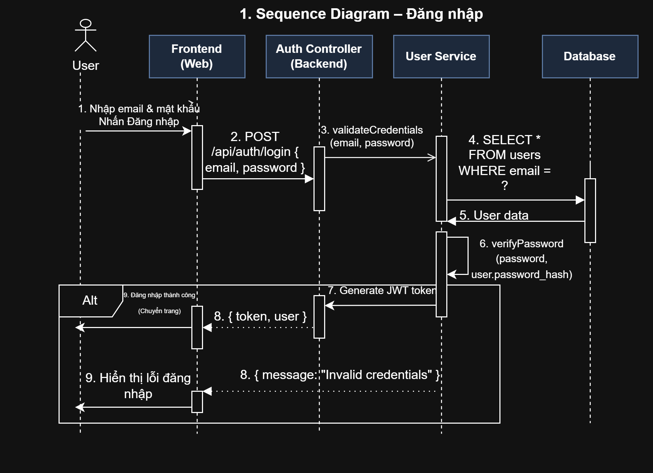
\includegraphics[width=\textwidth]{chuong3/images/sequence_login.png}
	\caption{Sequence Diagram chức năng Đăng nhập}
	\label{fig:sequence_login}
\end{figure}

%====================================================
\subsection{Sequence Diagram Nộp bài}
%====================================================

Chức năng nộp bài dự thi là một trong những chức năng quan trọng nhất của hệ thống SEAL Hackathon Management System. Sau khi đội thi hoàn thành sản phẩm, trưởng đội hoặc thành viên được cấp quyền có thể truy cập chức năng nộp bài để gửi sản phẩm tham gia cuộc thi. Toàn bộ quá trình nộp bài được thực hiện trực tuyến thông qua giao diện Web, giúp giảm thời gian xử lý và hỗ trợ Ban tổ chức quản lý tập trung các bài dự thi.

Quá trình bắt đầu khi người dùng lựa chọn chức năng nộp bài trên giao diện hệ thống. Người dùng nhập đầy đủ các thông tin theo yêu cầu như tên dự án, mô tả ngắn, đường dẫn GitHub và các thông tin liên quan đến sản phẩm. Trong trường hợp hệ thống hỗ trợ tải tệp đính kèm, người dùng cũng có thể lựa chọn các tệp cần nộp trước khi gửi yêu cầu đến máy chủ.

Trước khi dữ liệu được gửi đi, Frontend thực hiện kiểm tra sơ bộ nhằm đảm bảo các trường thông tin bắt buộc đã được nhập đầy đủ và đúng định dạng. Các lỗi như thiếu tên dự án, đường dẫn GitHub không hợp lệ hoặc dữ liệu không đúng định dạng sẽ được thông báo ngay trên giao diện, giúp giảm số lượng yêu cầu không hợp lệ gửi đến Backend.

Sau khi người dùng xác nhận nộp bài, Frontend gửi yêu cầu đến Submission Controller thông qua API tương ứng. Submission Controller tiếp nhận yêu cầu và tiến hành xác thực Access Token nhằm đảm bảo người gửi yêu cầu đã đăng nhập vào hệ thống. Nếu Token không hợp lệ hoặc đã hết hạn, hệ thống sẽ từ chối yêu cầu và yêu cầu người dùng đăng nhập lại.

Khi quá trình xác thực hoàn tất, Submission Controller tiếp tục chuyển dữ liệu đến tầng xử lý nghiệp vụ để thực hiện các bước kiểm tra cần thiết. Hệ thống xác định người dùng hiện tại có thuộc một đội thi hợp lệ hay không, kiểm tra quyền nộp bài của người dùng, đồng thời xác minh cuộc thi vẫn còn trong thời gian cho phép nộp bài. Đây là bước quan trọng nhằm đảm bảo chỉ những đội đủ điều kiện mới được phép gửi bài dự thi.

Nếu tất cả các điều kiện đều được đáp ứng, hệ thống tiến hành tạo bản ghi mới trong bảng Submission của cơ sở dữ liệu. Các thông tin như tên dự án, mô tả, đường dẫn GitHub, thời gian nộp và trạng thái bài nộp được lưu lại nhằm phục vụ quá trình đánh giá sau này. Trong trường hợp đội đã từng nộp bài trước đó, hệ thống có thể cập nhật bài nộp hoặc từ chối yêu cầu tùy theo quy định của cuộc thi.

Sau khi dữ liệu được lưu thành công, Backend gửi phản hồi về Frontend với thông báo nộp bài thành công. Giao diện hiển thị kết quả để người dùng xác nhận rằng hệ thống đã ghi nhận bài dự thi. Nếu xảy ra lỗi trong quá trình xử lý như mất kết nối cơ sở dữ liệu, dữ liệu không hợp lệ hoặc quá thời gian nộp bài, hệ thống sẽ trả về thông báo lỗi tương ứng để người dùng có thể thực hiện lại thao tác.

Thông qua Sequence Diagram của chức năng nộp bài có thể thấy rõ vai trò của từng thành phần trong hệ thống. Frontend chịu trách nhiệm thu thập dữ liệu và gửi yêu cầu, Submission Controller tiếp nhận và điều phối xử lý, tầng Service kiểm tra các quy tắc nghiệp vụ, còn Database chịu trách nhiệm lưu trữ thông tin bài dự thi. Việc phân chia nhiệm vụ rõ ràng giữa các thành phần giúp hệ thống hoạt động ổn định, dễ bảo trì và thuận tiện trong quá trình mở rộng.

\begin{figure}[H]
	\centering
	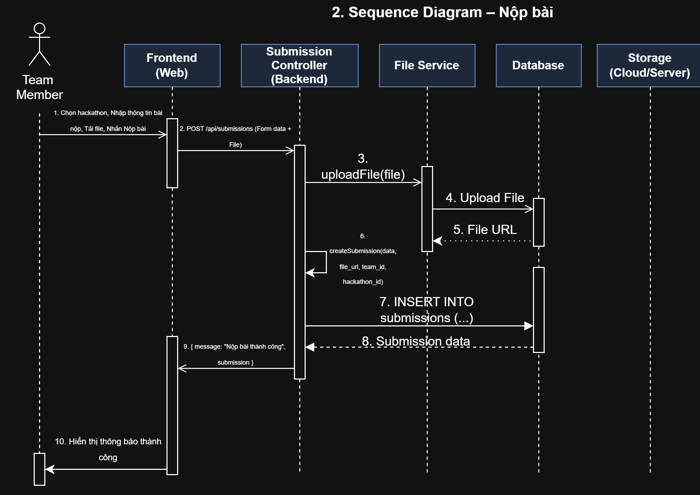
\includegraphics[width=\textwidth]{chuong3/images/sequence_submit.png}
	\caption{Sequence Diagram chức năng Nộp bài}
	\label{fig:sequence_submit}
\end{figure}

%====================================================
\subsection{Sequence Diagram Chấm điểm}
%====================================================

Sau khi kết thúc thời gian nhận bài, các giám khảo sẽ sử dụng chức năng chấm điểm để đánh giá các bài dự thi của từng đội. Chức năng này đóng vai trò quan trọng trong việc xác định kết quả cuối cùng của cuộc thi, vì vậy hệ thống yêu cầu người thực hiện phải được phân quyền với vai trò Judge trước khi có thể truy cập chức năng này.

Quá trình chấm điểm bắt đầu khi giám khảo đăng nhập vào hệ thống và truy cập danh sách các bài dự thi được phân công. Giao diện hiển thị đầy đủ thông tin về dự án như tên đội, tên dự án, mô tả, đường dẫn GitHub và các tài liệu liên quan nhằm hỗ trợ giám khảo trong quá trình đánh giá.

Sau khi lựa chọn bài dự thi cần chấm, giám khảo nhập điểm số theo các tiêu chí của cuộc thi và bổ sung nhận xét nếu cần thiết. Trước khi gửi dữ liệu, Frontend thực hiện kiểm tra nhằm đảm bảo điểm số nằm trong khoảng cho phép và các trường dữ liệu bắt buộc đã được nhập đầy đủ.

Khi người dùng nhấn nút xác nhận, Frontend gửi yêu cầu đến Score Controller thông qua API chấm điểm. Backend tiếp nhận yêu cầu và thực hiện xác thực Access Token nhằm đảm bảo người gửi yêu cầu đã đăng nhập và có vai trò giám khảo. Nếu người dùng không có quyền thực hiện chức năng này, hệ thống sẽ từ chối yêu cầu và trả về thông báo lỗi.

Sau khi hoàn thành bước xác thực, Score Controller chuyển dữ liệu đến tầng xử lý nghiệp vụ để kiểm tra tính hợp lệ của bài dự thi cũng như kiểm tra việc giám khảo đã thực hiện chấm bài trước đó hay chưa. Điều này giúp hạn chế việc lưu nhiều kết quả đánh giá trùng lặp đối với cùng một bài dự thi.

Nếu dữ liệu hợp lệ, hệ thống tiến hành tạo bản ghi mới trong bảng Score của cơ sở dữ liệu. Thông tin được lưu bao gồm mã bài dự thi, mã giám khảo, điểm số, nhận xét và thời gian thực hiện đánh giá. Trong một số trường hợp, hệ thống cũng có thể cập nhật điểm trung bình hoặc kết quả tổng hợp sau khi nhiều giám khảo hoàn thành việc chấm điểm.

Sau khi lưu dữ liệu thành công, Backend trả kết quả về Frontend và hiển thị thông báo chấm điểm thành công cho giám khảo. Trong trường hợp xảy ra lỗi như dữ liệu không hợp lệ, bài dự thi không tồn tại hoặc giám khảo không có quyền chấm điểm, hệ thống sẽ trả về thông báo phù hợp để người dùng xử lý.

Sequence Diagram của chức năng chấm điểm thể hiện đầy đủ quá trình tương tác giữa giám khảo, giao diện người dùng, Score Controller, tầng xử lý nghiệp vụ và cơ sở dữ liệu. Thông qua sơ đồ này có thể quan sát rõ trình tự xử lý dữ liệu từ khi giám khảo gửi yêu cầu cho đến khi kết quả đánh giá được lưu trữ thành công. Việc thiết kế theo mô hình nhiều tầng giúp đảm bảo tính nhất quán của dữ liệu, tăng khả năng bảo trì hệ thống và hỗ trợ mở rộng chức năng trong các phiên bản tiếp theo.

\begin{figure}[H]
	\centering
	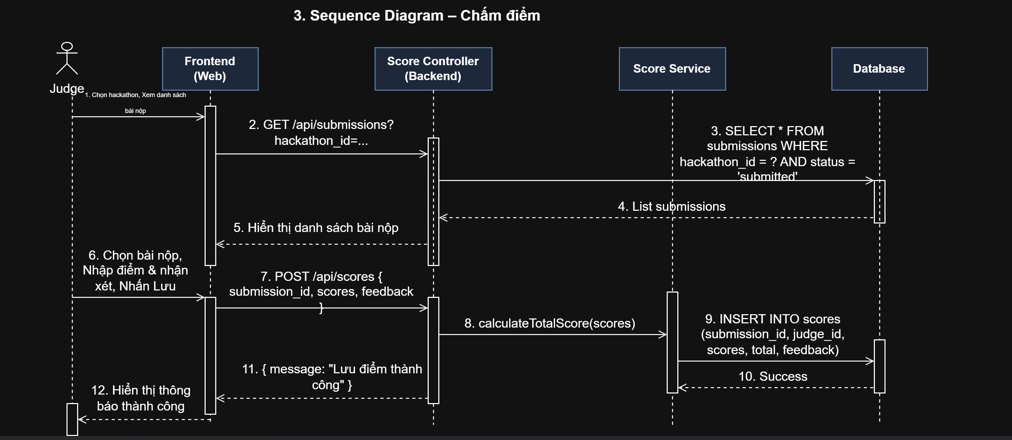
\includegraphics[width=\textwidth]{chuong3/images/sequence_score.png}
	\caption{Sequence Diagram chức năng Chấm điểm}
	\label{fig:sequence_score}
\end{figure}
